\documentclass[11pt]{charter}

% El títulos de la memoria, se usa en la carátula y se puede usar el cualquier lugar del documento con el comando \ttitle
\titulo{Control Automático de Ganancia para Sistema de Anuncios a Pasajeros} 

% Nombre del posgrado, se usa en la carátula y se puede usar el cualquier lugar del documento con el comando \degreename
\posgrado{Carrera de Especialización en Sistemas Embebidos} 
%\posgrado{Carrera de Especialización en Internet de las Cosas} 
%\posgrado{Carrera de Especialización en Intelegencia Artificial}
%\posgrado{Maestría en Sistemas Embebidos} 
%\posgrado{Maestría en Internet de las cosas}

% Tu nombre, se puede usar el cualquier lugar del documento con el comando \authorname
\autor{Ing. Gustavo Ramoscelli} 
\pertenenciaAutor{UNS}

% El nombre del director y co-director, se puede usar el cualquier lugar del documento con el comando \supname y \cosupname y \pertesupname y \pertecosupname
\director{Dr. Ing. Ariel Lutenberg}
\pertenenciaDirector{FIUBA, CONICET} 
% FIXME:NO IMPLEMENTADO EL CODIRECTOR ni su pertenencia
\codirector{} % si queda vacio no se deberíá incluir 
\pertenenciaCoDirector{}

% Nombre del cliente, quien va a aprobar los resultados del proyecto, se puede usar con el comando \clientename y \empclientename
\cliente{Ing. Martín Harris}
\empresaCliente{SOFSE}

% Nombre y pertenencia de los jurados, se pueden usar el cualquier lugar del documento con el comando \jurunoname, \jurdosname y \jurtresname y \perteunoname, \pertedosname y \pertetresname.
\juradoUno{Nombre y Apellido (1)}
\pertenenciaJurUno{pertenencia (1)} 
\juradoDos{Nombre y Apellido (2)}
\pertenenciaJurDos{pertenencia (2)}
\juradoTres{Nombre y Apellido (3)}
\pertenenciaJurTres{pertenencia (3)}
 
\fechaINICIO{22 de junio de 2020}		%Fecha de inicio de la cursada de GdP \fechaInicioName
\fechaFINALPlanificacion{22 de Agosto de 2020} 	%Fecha de final de cursada de GdP
\fechaFINALTrabajo{22 de diciembre de 2020}		%Fecha de defensa pública del trabajo final

\begin{document}

\maketitle
\thispagestyle{empty}
\pagebreak


\thispagestyle{empty}
{\setlength{\parskip}{0pt}
\tableofcontents{}
}
\pagebreak


\section{Registros de cambios}
\label{sec:registro}


\begin{table}[ht]
\label{tab:registro}
\centering
\begin{tabularx}{\linewidth}{@{}|c|X|c|@{}}
\hline
\rowcolor[HTML]{C0C0C0} 
Revisión & \multicolumn{1}{c|}{\cellcolor[HTML]{C0C0C0}Detalles de los cambios realizados} & Fecha      \\ \hline
1.0      & Creación del documento                                          & 27/06/2020 \\ \hline
1.1      &                                                                 & dd/mm/aaaa \\ \hline
1.2      &                                                                 & dd/mm/aaaa \\ \hline
\end{tabularx}
\end{table}

\pagebreak



\section{Acta de constitución del proyecto}
\label{sec:acta}

\begin{flushright}
Buenos Aires, \fechaInicioName
\end{flushright}

\vspace{2cm}

Por medio de la presente se acuerda con el Ing. \authorname\hspace{1px} que su Trabajo Final de la \degreename\hspace{1px} se titulará ``\ttitle'', consistirá en el prototipo preliminar de un sistema de control digital de volúmen, y tendrá un presupuesto preliminar estimado de 600 hs de trabajo, con fecha de inicio \fechaInicioName\hspace{1px} y fecha de presentación pública \fechaFinalName.

Se adjunta a esta acta la planificación inicial.

\vfill

% Esta parte se construye sola con la información que hayan cargado en el preámbulo del documento y no debe modificarla
\begin{table}[ht]
\centering
\begin{tabular}{ccc}
\begin{tabular}[c]{@{}c@{}}Ariel Lutenberg \\ Director posgrado FIUBA\end{tabular} &  & \begin{tabular}[c]{@{}c@{}}\clientename \\ \empclientename \end{tabular} \vspace{2.5cm} \\ 
\multicolumn{3}{c}{\begin{tabular}[c]{@{}c@{}} \supname \\ Director del Trabajo Final\end{tabular}} \vspace{2.5cm} \\
\begin{tabular}[c]{@{}c@{}}\jurunoname \\ Jurado del Trabajo Final\end{tabular}     &  & \begin{tabular}[c]{@{}c@{}}\jurdosname\\ Jurado del Trabajo Final\end{tabular}  \vspace{2.5cm}  \\
\multicolumn{3}{c}{\begin{tabular}[c]{@{}c@{}} \jurtresname\\ Jurado del Trabajo Final\end{tabular}} \vspace{.5cm}                                                                     
\end{tabular}
\end{table}




\section{Descripción técnica-conceptual del proyecto a realizar}
\label{sec:descripcion}

El presente proyecto busca solucionar un problema que ocasiona quejas frecuentes por parte de los pasajeros de 
distintas líneas de trenes de la Argentina: la dificultad de escuchar correctamente los 
anuncios que se reproducen por los altoparlantes de los trenes en movimiento. Debido al ruido 
ambiente producido por distintas fuentes como por ejemplo: los propios pasajeros, los ruidos 
mecánicos de la formación y los ruidos externos, en diversos puntos del recorrido se hace necesario 
aumentar el volúmen del sistema de anuncios por audio ({\em audio announcement system \/} en inglés)
en ciertas partes del viaje. Sin embargo, aumentar demasiado el volumen puede producir una sensación 
de aturdimiento, especialmente en tramos donde el nivel de ruido ambiente es menor. Por esto es deseable 
instalar en las formaciones un {\em control automático de ganacia\/} (CAG). 

Existen en el mercado internacional soluciones comerciales con prestaciones similares a las ofrecidas por 
este proyecto, como por ejemplo este producto de fabricación extranjera: \href{http://www.ervocom.ch/en/module/solutions/10-digital-audio-solution-for-passenger-announcements}
{Passenger announcement for rolling stock}. Sin embargo, hay varios motivos para desarrollar una solución nacional. Un
motivo es el costo elevado de  los productos ferroviarios de importación respecto de los productos
nacionales. Otro motivo es que las soluciones comerciales de productos
ferroviarios en general usan tecnologías diferentes a las usadas en las formaciones locales lo que 
implica hacer complejas adaptaciones del producto. Estos motivos justifican  la reallización del presente proyecto. 

\vspace{25px}

\begin{figure}[htpb]
\centering 
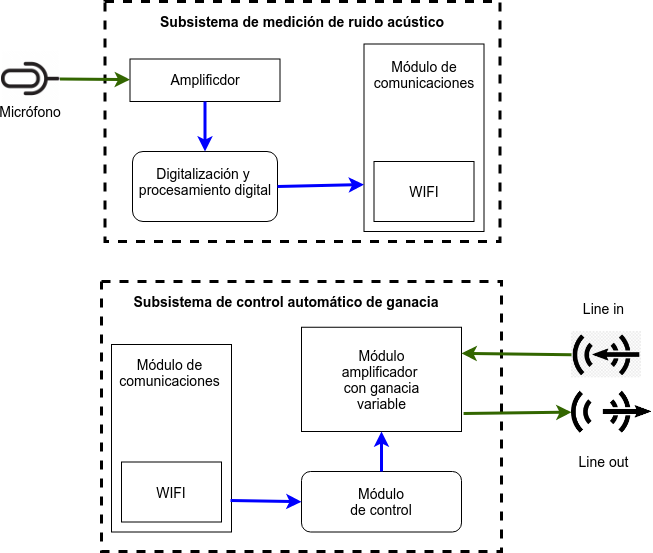
\includegraphics[width=.7\textwidth]{./Figuras/arqCAG.png}
\caption{Diagrama en bloques de la arquitectura del sistema CAG }
\label{fig:diagBloques}
\end{figure}

\vspace{25px}

Como se observa en la Fig. \ref{fig:diagBloques} el sistema a implementar está compuesto por dos subsistemas. Uno es el subsistema de medición de ruido ambiente que se encarga de obtener el nivel de ruido acústico del lugar donde está instalado para luego enviar este dato a travez de una red {\em mesh\/} de sensores. Se instalarán varios de estos subsistemas por cada formación de tren.

El subsistema de control automático de ganacia recibe a travez de la red de sensores los niveles de ruido de cada punto de medición
y con estos datos ajusta el nivel de la señal de audio que proviene del sistema de anuncios y que se envía a los altoparlantes del tren.  


\section{Identificación y análisis de los interesados}
\label{sec:interesados}

\begin{table}[ht]
%\caption{Identificación de los interesados}
%\label{tab:interesados}
\begin{tabularx}{\linewidth}{@{}|l|X|X|l|@{}}
\hline
\rowcolor[HTML]{C0C0C0} 
Rol           & Nombre y Apellido & Organización 	& Puesto 	\\ \hline
Cliente       & \clientename      &\empclientename	&   Coordinador General
de Desarrollo     	\\ \hline
Responsable   & \authorname       & FIUBA        	& Alumno 	\\ \hline
Orientador    & \supname	      & \pertesupname 	& Director	Trabajo final \\ \hline
Usuario final &                   &              	&        	\\ \hline
\end{tabularx}
\end{table}

El Ing. Martin Harris se ofreció a comprar el material necesario.

El Ing. Ariel Lutenberg se comprometió a realizar las gestiones de ingreso del proyecto en SOFSE para su aprobación. Muchas veces no está disponible por su apretada agenda.

\section{1. Propósito del proyecto}
\label{sec:proposito}

El propósito de este proyecto consiste en desarrollar un sistema de control automático de ganacia del sistema de anuncios de audio de las formaciones de trenes. Tiene dos objetivos principales:
\begin{itemize}
\item Mejorar la calidad del audio de los anuncios a los pasajeros.
\item Enviar los datos de reuido georeferenciados a los servidores de SOFSE para su análisis y registración.
\end{itemize}

\section{2. Alcance del proyecto}
\label{sec:alcance}

Los dispositivos a desarrollar serán dos: el dispositivo de medición de ruido ambiente y el dispositivo de control automático de ganacia.
El dispositivo de medición de ruido acústico obtendrá el dato del nivel de ruido acústico a partir del procesamiento de la señal de audio capatada por un micrófono. Luego transmitirá el dato del nivel de ruido acústico a través de una red {\em mesh\/} a un servidor central y al dispositvo del subsistema de control automático de ganacia.

El dispositivo que realiza el control automático de ganacia recibe el dato del nivel de ruido de todos los dispositivos de medición de ruido acústico instalados en la formación. Usando los datos de ruido acústico realizará el ajuste necesario en la ganacia de un amplificador de audio interno. Además el dispositivo tendrá una entrada de audio y una salida de audio. La entrada de audio del dipositivo estará conectada a la señal de audio del sistema de anuncios del tren y la salida de audio estará conectada a los parlantes instalados en el tren.

El sistema propuesto que se muestra en la Fig. \ref{fig:diagBloques} tiene  como meta a alcanzar  la implementación de los componentes de abajo:

\begin{itemize}
\item Desarrollo de firmware para microcontrolador del módulo principal del sistema.
\item Desarrollo de firmware para microcontrolador del módulo de comunicaciones WIFI.
\item Desarrollo de interfaz web responsiva que será provista por el módulo de comunicaciones
para la configuración.
\item Diseño de hardware para el sistema.
\item Prototipo funcional.
No estará contemplado por este proyecto:
\item El software de PC de análisis de la información recolectada.
\end{itemize}

\section{3. Supuestos del proyecto}
\label{sec:supuestos}

Para el presente proyecto se consideran con los siguientes supuestos:
\begin{itemize}
\item Para el desarrollo del módulo principal se utilizará una solución microprocesada basada en
EDU-CIA, debido que se tiene disponibilidad de la misma y posee un procesador de tipo,
arquitectura y modelos ampliamente utilizados en proyectos de sistemas embebidos.
\item Para el desarrollo del módulo de comunicaciones WIFI se utilizará una solución basada un módulo de la familia ESP32, debido a que es ampliamente utilizado en internet de las cosas, y como interfaces integrantes de soluciones de sistemas embebidos.
\end{itemize}
\section{4. Requerimientos}
\label{sec:requerimientos}

Los requerimientos para el presente proyecto son los enumerados abajo:
\begin{enumerate}
\item Grupo de requerimientos del subsistema de medición de ruido acústico.
  \begin{enumerate}
  \item Adecuación del nivel de señal de audio capatado por el micrófono para mejorar el rango dinámico en la digitalización de la señal por parte del conversor ADC.
  \item Obtención del nivel de ruido acústico  mediante el procesamiento digital de la señal digital proveniente del conversor ADC.
  \item Envío de los niveles de ruido acústico en tiempo real a un servidor remoto por paquetes MQTT mediante protocolo seguro (TLS).
  \item Almacenamiento local de los datos enviados (backup)
  \item Actualización del {\em firmware\/} completo por WIFI.  \item Configuración general del subsistema por página web.
  \item Configuración general del sistema por mensajes MQTT.
  \end{enumerate}
  
\item Grupo de requerimientos del subsistema de
control automático de ganacia.
  \begin{enumerate}
  \item Ajuste automático del nivel de ganancia del amplificador interno de audio en tiempo real en función de los valores de ruido ambiente reportados y de los valores de la configuración.
  \item Actualización del {\em firmware\/} completo por WIFI.
  \item Configuración general del subsistema por página web.
  \item Configuración general del sistema por mensajes MQTT.
  \end{enumerate}
  
\item Requerimientos generales
  \begin{enumerate}
  \item La alimentación deberá ser de 5V continua.
  \end{enumerate}
\item Grupo de requerimientos referidos a la interfaz de usuario.
  \begin{enumerate}
  \item Se deberá poder visualizar en la interfaz WIFI el estado del dispositivo, memoria disponible, valores de configuración, etc.
  \item Se deberá poder configurar ciertos parámetros de configuración funcionales como
ser la calibración del nivel de ruido acústico.
  \item Se deberá poder configurar parámetros de configuración referente a la conexión WIFI
(Red, Tópico, Usuario y Clave del Servidor MQTT, Certificado SSL, etc).
  \item Se deberá poder descargar las capturas en formato CSV de forma total o por rango
temporal.
  \end{enumerate}
\end{enumerate}

\section{Historias de usuarios (\textit{Product backlog})}
\label{sec:backlog}

\begin{consigna}{red}
Descripción: En esta sección se deben incluir las historias de usuarios y su ponderación (\textit{history points}). Recordar que las historias de usuarios son descripciones cortas y simples de una característica contada desde la perspectiva de la persona que desea la nueva capacidad, generalmente un usuario o cliente del sistema. La ponderación es un número entero que representa el tamaño de la historia comparada con otras historias de similar tipo.
\end{consigna}

\section{5. Entregables principales del proyecto}
\label{sec:entregables}

\begin{itemize}
\item Manual de uso.
\item Código fuente de firmware del módulo principal y de comunicaciones de todos los subsistemas.
\item Diseño de hardware de todos los subsistemas.
\item Documentación de arquitectura y diseño para transferencia de conocimiento que posibilite
futuras mejoras por parte del cliente.
\end{itemize}

\section{6. Desglose del trabajo en tareas}
\label{sec:wbs}

\begin{enumerate}
\item Grupo de tareas iniciales
	\begin{enumerate}
	\item Realizar el plan del proyecto (12 hs).
	\item Ingeniería de detalle: se buscan los componentes electrónicos apropiados para la solución propuesta y se realizan las elecciones de los mismos. (24 hs)
	\item Investigar sobre procesamiento digital de señales de audio y elegir la mejor solución para la solución propuesta. (12 hs)
	\end{enumerate}
\item Grupo de tareas de la construcción de hardware
	\begin{enumerate}
	\item Diseño del hardware: Se realiza el diseño de la placa electrónica, el diagrama de
bloques detallado y los esquemáticos necesarios. (40 hs)
    \item Simulación del hardware: Se realiza la simulación del hardware diseñado para encontrar los valores óptimos de los componentes analógicos. (24 hs)
    \item Ruteo de pistas del PCB: Diseño de las placas PCB necesarias, mejoramiento de las especificaciones en función de los parámetros electrónicos y su adecuación para manufacturabilidad. (40 hs)
    \item Compra de componentes: Se buscará que todos los componentes electrónicos se encuentren en el mercado local. El tiempo puede ser mayor ante la necesidad de importarlos por falta de disponibilidad local. (4 hs + 30 días)
    \item Fabricación del PCB: Como el proyecto es un prototipo se realizará la manufactura artesanal del PCB. (12 hs).
    \item Montaje hardware: Montaje de componentes, soldadura manual y posiblemente en horno de los componentes SMD. (20 hs)
    \item Verificación hardware: Se realizan las pruebas neesarias sobre las placas armadas para asegurar su confiabilidad. (8 hs).
	\end{enumerate}
\item Grupo de tareas de la construcción del software
	\begin{enumerate}
	\item Diseño del software: Se realizan el documentos de requerimientos de software, el documento de arquitectura de software y se documenta la planificación del trabajo para seguir un desarrollo guiado por comportamiento. (24 hs)
    \item Implementación y testing del módulo de comunicaciones WIFI: Se realiza la integración de varias bibliotecas (protocoplo MQTT, protocolo HTTP, capa de seguridad TLS, etc). (8 hs).
    \item Maquetado e implementación de páginas Web: Se realiza el armado de las páginas Web para la configuración de distintos módulos y la presentación de información del sistema. (16 hs).
    \item Implementación del módulo de procesamiento digital de audio: Se realiza la implementación de filtros para la adecuación de la señal de audio digitalizada y la implemtación de algoritmos de procesamiento digital como FFT y otros. (40 hs).
    \item Módulo de ganancia automática: Implementación del módulo que a partir de los datos de ruido acústico y de configuración, entrega el nivel de ganancia a aplicar al amplificador analógico. (8 hs)
    \item Módulo de almacenamiento: Se reañliza la implementación del driver del filesystem de
memoria SD para almacenar el respaldos de los datos enviados por MQTT. (40 hs)
        \item Integración del sistema: Se realiza la implementación de las pruebas de integración de los distintos subsistemas y se llevan a cabo. Luego se integran todos los módulos. (40 hs)
	\end{enumerate}
\item Grupo de tareas de integración y validación
    \begin{enumerate}
    \item Integración Software con Hardware: Se integra el software funcionando en el
hardware manufacturado. (24 hs).
    \item Validación: Se realizan validaciones del producto, incluyendo pruebas de campo. (40
hs)
    \item Documentación: Se integrará la documentación tanto de las etapas de la fabricación
del producto, como los archivos de diseño. Adicionalmente se confeccionara los
manuales de uso del producto. (32 hs)
    \item Presentación: Se elaborará la presentación final del proyecto. (32 hs)
    \end{enumerate}
\end{enumerate}

Cantidad total de horas: (524 hs de trabajo + 30 días calendario de demora)


\section{7. Diagrama de Activity On Node}
\label{sec:AoN}

\begin{figure}[htpb]
\centering 
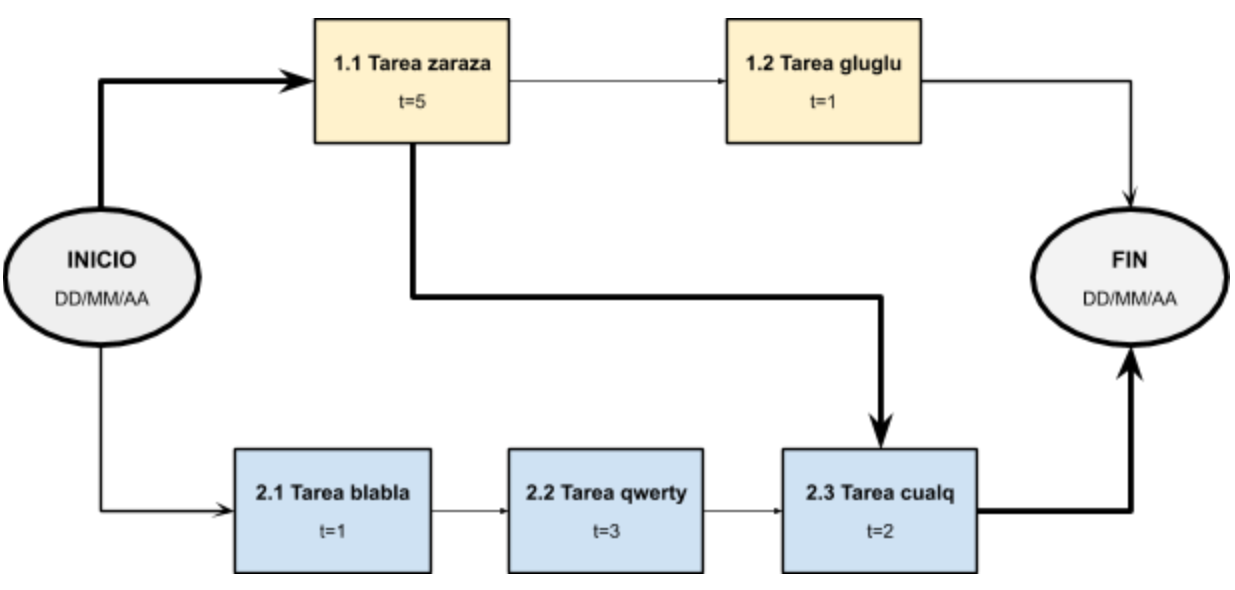
\includegraphics[width=.8\textwidth]{./Figuras/AoN.png}
\caption{Diagrama en \textit{Activity on Node}}
\label{fig:AoN}
\end{figure}


\section{8. Diagrama de Gantt}
\label{sec:gantt}

\begin{consigna}{red}
Utilizar el software Gantter for Google Drive o alguno similar para dibujar el diagrama de Gantt.

Existen muchos programas y recursos \textit{online} para hacer diagramas de gantt, entre las cuales destacamos:

\begin{itemize}
\item Planner
\item GanttProject
\item Trello + \textit{plugins}. En el siguiente link hay un tutorial oficial: \\ \url{https://blog.trello.com/es/diagrama-de-gantt-de-un-proyecto}
\item Creately, herramienta online colaborativa. \\\url{https://creately.com/diagram/example/ieb3p3ml/LaTeX}
\item Se puede hacer en latex con el paquete \textit{pgfgantt}\\ \url{http://ctan.dcc.uchile.cl/graphics/pgf/contrib/pgfgantt/pgfgantt.pdf}
\end{itemize}

Pegar acá una captura de pantalla del diagrama de Gantt, cuidando que la letra sea suficientemente grande como para ser legible. 
Si el diagrama queda demasiado ancho, se puede pegar primero la ``tabla'' del Gantt y luego pegar la parte del diagrama de barras del diagrama de Gantt.

Configurar el software para que en la parte de la tabla muestre los códigos del EDT (WBS).\\
Configurar el software para que al lado de cada barra muestre el nombre de cada tarea.\\
Revisar que la fecha de finalización coincida con lo indicado en el Acta Constitutiva.

En la figura \ref{fig:gantt}, se muestra un ejemplo de diagrama de gantt realizado con el paquete de \textit{pgfgantt}. En la plantilla pueden ver el código que lo genera y usarlo de base para construir el propio.

\begin{figure}[htbp]
\begin{center}
\begin{ganttchart}{1}{12}
  \gantttitle{2020}{12} \\
  \gantttitlelist{1,...,12}{1} \\
  \ganttgroup{Group 1}{1}{7} \\
  \ganttbar{Task 1}{1}{2} \\
  \ganttlinkedbar{Task 2}{3}{7} \ganttnewline
  \ganttmilestone{Milestone o hito}{7} \ganttnewline
  \ganttbar{Final Task}{8}{12}
  \ganttlink{elem2}{elem3}
  \ganttlink{elem3}{elem4}
\end{ganttchart}
\end{center}
\caption{Diagrama de gantt de ejemplo}
\label{fig:gantt}
\end{figure}

\end{consigna}

\section{9. Matriz de uso de recursos de materiales}
\label{sec:recursos}


\begin{table}[htpb]
\label{tab:recursos}
\centering
\begin{tabularx}{\linewidth}{@{}|c|X|X|X|X|X|@{}}
\hline
\cellcolor[HTML]{C0C0C0} & \cellcolor[HTML]{C0C0C0} & \multicolumn{4}{c|}{\cellcolor[HTML]{C0C0C0}Recursos requeridos (horas)} \\ \cline{3-6} 
\multirow{-2}{*}{\cellcolor[HTML]{C0C0C0}\begin{tabular}[c]{@{}c@{}}Código\\ WBS\end{tabular}} & \multirow{-2}{*}{\cellcolor[HTML]{C0C0C0}\begin{tabular}[c]{@{}c@{}}Nombre \\ tarea\end{tabular}} & Material 1 & Material 2 & Material 3 & Material 4 \\ \hline
 &  &  &  &  &  \\ \hline
 &  &  &  &  &  \\ \hline
 &  &  &  &  &  \\ \hline
 &  &  &  &  &  \\ \hline
\end{tabularx}%
\end{table}


\section{10. Presupuesto detallado del proyecto}
\label{sec:presupuesto}

\begin{table}[htpb]
\centering
\begin{tabularx}{\linewidth}{@{}|X|c|r|r|@{}}
\hline
\rowcolor[HTML]{C0C0C0} 
\multicolumn{•}{•}{•}umn{4}{|c|}{\cellcolor[HTML]{C0C0C0}COSTOS DIRECTOS} \\ \hline
\rowcolor[HTML]{C0C0C0} 
Descripción &
  \multicolumn{1}{c|}{\cellcolor[HTML]{C0C0C0}Cantidad} &
  \multicolumn{1}{c|}{\cellcolor[HTML]{C0C0C0}Valor unitario} &
  \multicolumn{1}{c|}{\cellcolor[HTML]{C0C0C0}Valor total} \\ \hline
 &
  \multicolumn{1}{c|}{} &
  \multicolumn{1}{c|}{} &
  \multicolumn{1}{c|}{} \\ \hline
 &
  \multicolumn{1}{c|}{} &
  \multicolumn{1}{c|}{} &
  \multicolumn{1}{c|}{} \\ \hline
\multicolumn{1}{|l|}{} &
   &
   &
   \\ \hline
\multicolumn{1}{|l|}{} &
   &
   &
   \\ \hline
\multicolumn{3}{|c|}{SUBTOTAL} &
  \multicolumn{1}{c|}{} \\ \hline
\rowcolor[HTML]{C0C0C0} 
\multicolumn{4}{|c|}{\cellcolor[HTML]{C0C0C0}COSTOS INDIRECTOS} \\ \hline
\rowcolor[HTML]{C0C0C0} 
Descripción &
  \multicolumn{1}{c|}{\cellcolor[HTML]{C0C0C0}Cantidad} &
  \multicolumn{1}{c|}{\cellcolor[HTML]{C0C0C0}Valor unitario} &
  \multicolumn{1}{c|}{\cellcolor[HTML]{C0C0C0}Valor total} \\ \hline
\multicolumn{1}{|l|}{} & asdfsdaf
   &
   &
   \\ \hline
\multicolumn{1}{|l|}{} &
   &
   &
   \\ \hline
\multicolumn{1}{|l|}{} &
   &
   &
   \\ \hline
\multicolumn{3}{|c|}{SUBTOTAL} &
  \multicolumn{1}{c|}{} \\ \hline
\rowcolor[HTML]{C0C0C0}
\multicolumn{3}{|c|}{TOTAL} &
   \\ \hline
\end{tabularx}%
\end{table}


\section{11. Matriz de asignación de responsabilidades}
\label{sec:responsabilidades}
\begin{consigna}{red}
Establecer la matriz de asignación de responsabilidades y el manejo de la autoridad completando la siguiente tabla:

\begin{table}[htpb]
\centering
\resizebox{\textwidth}{!}{%
\begin{tabular}{|c|c|c|c|c|c|}
\hline
\rowcolor[HTML]{C0C0C0} 
\cellcolor[HTML]{C0C0C0} &
  \cellcolor[HTML]{C0C0C0} &
  \multicolumn{4}{c|}{\cellcolor[HTML]{C0C0C0}Listar todos los nombres y roles del proyecto} \\ \cline{3-6} 
\rowcolor[HTML]{C0C0C0} 
\cellcolor[HTML]{C0C0C0} &
  \cellcolor[HTML]{C0C0C0} &
  Responsable &
  Orientador &
  Equipo &
  Cliente \\ \cline{3-6} 
\rowcolor[HTML]{C0C0C0} 
\multirow{-3}{*}{\cellcolor[HTML]{C0C0C0}\begin{tabular}[c]{@{}c@{}}Código\\ WBS\end{tabular}} &
  \multirow{-3}{*}{\cellcolor[HTML]{C0C0C0}Nombre de la tarea} &
  \authorname &
  \supname &
  Nombre de alguien &
  \clientename \\ \hline
 &  &  &  &  &  \\ \hline
 &  &  &  &  &  \\ \hline
 &  &  &  &  &  \\ \hline
\end{tabular}%
}
\end{table}

{\footnotesize
Referencias:
\begin{itemize}
	\item P = Responsabilidad Primaria
	\item S = Responsabilidad Secundaria
	\item A = Aprobación
	\item I = Informado
	\item C = Consultado
\end{itemize}
} %footnotesize

Una de las columnas debe ser para el Director, ya que se supone que participará en el proyecto.
A su vez se debe cuidar que no queden muchas tareas seguidas sin ``A'' o ``I''.

Importante: es redundante poner ``I/A'' o ``I/C'', porque para aprobarlo o responder consultas primero la persona debe ser informada.

\end{consigna}

\section{12. Gestión de riesgos}
\label{sec:riesgos}

\begin{consigna}{red}
a) Identificación de los riesgos (al menos cinco) y estimación de sus consecuencias:
 
Riesgo 1: detallar el riesgo (riesgo es algo que si ocurre altera los planes previstos)
\begin{itemize}
\item Severidad (S): mientras más severo, más alto es el número (usar números del 1 al 10).\\
Justificar el motivo por el cual se asigna determinado número de severidad (S).
\item Probabilidad de ocurrencia (O): mientras más probable, más alto es el número (usar del 1 al 10).\\
Justificar el motivo por el cual se asigna determinado número de (O). 
\end{itemize}   

Riesgo 2:
\begin{itemize}
\item Severidad (S): 
\item Ocurrencia (O):
\end{itemize}

Riesgo 3:
\begin{itemize}
\item Severidad (S): 
\item Ocurrencia (O):
\end{itemize}


b) Tabla de gestión de riesgos:      (El RPN se calcula como RPN=SxO)

\begin{table}[htpb]
\centering
\begin{tabularx}{\linewidth}{@{}|X|c|c|c|c|c|c|@{}}
\hline
\rowcolor[HTML]{C0C0C0} 
Riesgo & S & O & RPN & S* & O* & RPN* \\ \hline
       &   &   &     &    &    &      \\ \hline
       &   &   &     &    &    &      \\ \hline
       &   &   &     &    &    &      \\ \hline
       &   &   &     &    &    &      \\ \hline
       &   &   &     &    &    &      \\ \hline
\end{tabularx}%
\end{table}

Criterio adoptado: 
Se tomarán medidas de mitigación en los riesgos cuyos números de RPN sean mayores a ....

Nota: los valores marcados con (*) en la tabla corresponden luego de haber aplicado la mitigación.

c) Plan de mitigación de los riesgos que originalmente excedían el RPN máximo establecido:
 
Riesgo 1: Plan de mitigación (si por el RPN fuera necesario elaborar un plan de mitigación).
  Nueva asignación de S y O, con su respectiva justificación:
  - Severidad (S): mientras más severo, más alto es el número (usar números del 1 al 10).
          Justificar el motivo por el cual se asigna determinado número de severidad (S).
  - Probabilidad de ocurrencia (O): mientras más probable, más alto es el número (usar del 1 al 10).
          Justificar el motivo por el cual se asigna determinado número de (O).

Riesgo 2: Plan de mitigación (si por el RPN fuera necesario elaborar un plan de mitigación).
 
Riesgo 3: Plan de mitigación (si por el RPN fuera necesario elaborar un plan de mitigación)

\end{consigna}


\section{13. Gestión de la calidad}
\label{sec:calidad}

\begin{consigna}{red}
Para cada uno de los requerimientos del proyecto indique:
\begin{itemize} 
\item Req \#1: Copiar acá el requerimiento.

Verificación y validación:

\begin{itemize}
\item Verificación para confirmar si se cumplió con lo requerido antes de mostrar el sistema al cliente:\\
Detallar 
\item Validación con el cliente para confirmar que está de acuerdo en que se cumplió con lo requerido:\\
Detallar  
\end{itemize}

\end{itemize}

Tener en cuenta que en este contexto se pueden mencionar simulaciones, cálculos, revisión de hojas de datos, consulta con expertos, etc.

\end{consigna}

\section{14. Comunicación del proyecto}
\label{sec:comunicaciones}

\begin{consigna}{red}
El plan de comunicación del proyecto es el siguiente:
\end{consigna}

% Please add the following required packages to your document preamble:
% \usepackage{graphicx}
% \usepackage[table,xcdraw]{xcolor}
% If you use beamer only pass "xcolor=table" option, i.e. \documentclass[xcolor=table]{beamer}
\begin{table}[htpb]
\centering
\resizebox{\textwidth}{!}{%
\begin{tabular}{|c|c|c|c|c|c|}
\hline
\rowcolor[HTML]{C0C0C0} 
\multicolumn{6}{|c|}{\cellcolor[HTML]{C0C0C0}PLAN DE COMUNICACIÓN DEL PROYECTO}           \\ \hline
\rowcolor[HTML]{C0C0C0} 
¿Qué comunicar? & Audiencia & Propósito & Frecuencia & Método de comunicac. & Responsable \\ \hline
                &           &           &            &                      &             \\ \hline
                &           &           &            &                      &             \\ \hline
                &           &           &            &                      &             \\ \hline
                &           &           &            &                      &             \\ \hline
                &           &           &            &                      &             \\ \hline
\end{tabular}%
}
\end{table}

\section{15. Gestión de compras}
\label{sec:compras}

\begin{consigna}{red}
En caso de tener que comprar elementos o contratar servicios:
a) Explique con qué criterios elegiría a un proveedor.
b) Redacte el Statement of Work correspondiente.
\end{consigna}

\section{16. Seguimiento y control}
\label{sec:seguimiento}

\begin{consigna}{red}
Para cada tarea del proyecto establecer la frecuencia y los indicadores con los se seguirá su avance y quién será el responsable de hacer dicho seguimiento y a quién debe comunicarse la situación (en concordancia con el Plan de Comunicación del proyecto).

El indicador de avance tiene que ser algo medible, mejor incluso si se puede medir en \% de avance. Por ejemplo,se pueden indicar en esta columna cosas como ``cantidad de conexiones ruteadeas'' o ``cantidad de funciones implementadas'', pero no algo genérico y ambiguo como ``\%'', porque el lector no sabe porcentaje de qué cosa.

\end{consigna}

\begin{table}[!htpb]
\centering
\begin{tabularx}{\linewidth}{@{}|X|X|X|X|X|X|@{}}
\hline
\rowcolor[HTML]{C0C0C0} 
\multicolumn{6}{|c|}{\cellcolor[HTML]{C0C0C0}SEGUIMIENTO DE AVANCE}                                                                       \\ \hline
\rowcolor[HTML]{C0C0C0} 
Tarea del WBS & Indicador de avance & Frecuencia de reporte & Resp. de seguimiento & Persona a ser informada & Método de comunic. \\ \hline
 &  &  &  &  &  \\ \hline
 &  &  &  &  &  \\ \hline
 &  &  &  &  &  \\ \hline
 &  &  &  &  &  \\ \hline
 &  &  &  &  &  \\ \hline
\end{tabularx}%
%}
\end{table}

\section{17. Procesos de cierre}    
\label{sec:cierre}

\begin{consigna}{red}
Establecer las pautas de trabajo para realizar una reunión final de evaluación del proyecto, tal que contemple las siguientes actividades:

\begin{itemize}
\item Pautas de trabajo que se seguirán para analizar si se respetó el Plan de Proyecto original:
 - Indicar quién se ocupará de hacer esto y cuál será el procedimiento a aplicar. 
\item Identificación de las técnicas y procedimientos útiles e inútiles que se utilizaron, y los problemas que surgieron y cómo se solucionaron:
 - Indicar quién se ocupará de hacer esto y cuál será el procedimiento para dejar registro.
\item Indicar quién organizará el acto de agradecimiento a todos los interesados, y en especial al equipo de trabajo y colaboradores:
  - Indicar esto y quién financiará los gastos correspondientes.
\end{itemize}

\end{consigna}


\end{document}
